\section{Advanced retrieval models}
\subsection{Latent semantic indexing}
Vector Space Retrieval not ideal, vague and noisy. Information needed is more related to \emph{concepts}, ideas than to index terms.

Unable to handle \emph{synonymy} (result: poor recall) and \emph{homonymy} (result: poor precision).

Map documents and queries to lower-\emph{dimensional}, higher-\emph{level} \textbf{concept space}. Each concept is represented by \emph{a combination of terms}. The concepts become an \emph{intermediate layer} between terms and documents.

\subsubsection{Similarity computation} With concepts represented by sets of terms, documents are represented by a concept vector, counting the number of concept terms. Similarity is computed by \emph{scalar product} of normalized concept vectors (cosine similarity).

Concepts could be identified manually by using defined ontology and users annotating documents. Instead, \textbf{use term-document matrix} $\mathbf{M_{ij}}$ with $m$ rows (terms $k_i$, $n$ columns (documents $d_j$). Weights based on \emph{tf-idf}.

\begin{figure}
  \centering
  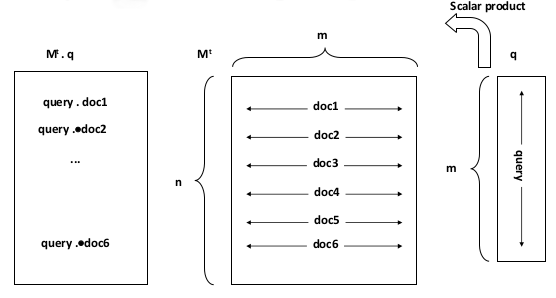
\includegraphics[width=\linewidth]{figures/computing_ranking.png}
  \caption{Product of normalized document-term matrix $M^T$ and query vector $\vec{q}$ to compute ranking.}
  \label{fig:computing_ranking}
\end{figure}

Let $\vec{q}$ be the query vector of size $m$ with a weight for each term $k_i$ and $M^T$ the transposed term-document matrix, s.t. each row represents a document. Producing retrieval results is shown in \cref{fig:computing_ranking}

\subsubsection{Singular Value Decomposition}

\subsection{Word Embeddings}
